\chapter{Détection de groupes pertinents dans les flots de liens}
\minitoc

\label{groupesDense}
Nous avons vu précédemment qu'il est possible de trouver des groupes de liens dans un flots de liens via l'intermédiaire d'une projection du flot de liens en un graphe statique.
Pour ce faire, nous avons appliqué l'algorithme de Louvain sur la projection pour obtenir une partition des liens en communautés.
Parmi l'ensemble des communautés, il se peut que certaines capturent des structures plus importantes et plus pertinentes que d'autres.
Le but ici est de réussir à extraire parmi ces groupes ceux qui sont pertinents.
En ce sens, nous nous posons la question de la décomposition partielle d'un flot de liens en sous-flots pertinents.
Il s'agit donc d'un problème légèrement différent de la détection de partition car d'une part, certains liens peuvent n'appartenir à aucun groupe et, d'autre part, les groupes doivent être pertinents.

Toute la difficulté pour réussir à trouver les groupes pertinents est de trouver une définition de la pertinence.
La notion de densité, que nous avons utilisée précédemment, est une première approche mais ce n'est pas suffisant.
En effet, il peut exister de grand groupes pertinents mais peu denses et de petits groupes très denses mais peu pertinents.
Il n'est pas possible de faire la différence entre ces deux catégories en utilisant juste la densité.
C'est pourquoi, nous utilisons une notion de voisinage.
Un groupe est alors pertinent s'il est plus dense que son voisinage.
Ainsi, un groupe peu dense peut être pertinent s'il est plus dense que son voisinage.
Comme le but est de pouvoir décrire le flot de liens, nous nous limitons aux groupes ayant une taille supérieur à un minimum donné.
Un exemple de flots avec une décomposition en groupes pertinents est dans la figure~\ref{fig:exemple_groupe_dens}.

Afin de trouver des groupes pertinents, nous procédons de la manière suivantes:
\begin{itemize}
\item Nous construisons la projection du flot de liens en un graphe statique;
\item Nous appliquons sur cette projection un algorithme de détection de communautés afin d'obtenir une partition des liens du flot de liens;
\item Nous ne gardons dans la partition que les groupes qui sont considérés comme pertinents, c'est-à-dire ceux qui sont assez gros et qui sont plus denses que leur voisinage.
\end{itemize}

Afin de montrer la pertinence de cette approche, nous l'appliquons sur différents jeux de données et faisons une analyse manuelle de certains groupes trouvés.
Par ailleurs, nous montrons que les groupes que nous détectons ne le sont pas par une méthode statique.

Le chapitre est organisé de la manière suivante.
Dans la section~\ref{sec:groupe_dense_existant}, nous revenons sur les travaux existants qui traitent de sujets similaires.
Puis dans la section~\ref{sec:groupe_dense_method}, nous présentons notre méthode de détection et de validation de groupes pertinents.
Enfin, les jeux de données que nous utilisons sont présentés dans la section~\ref{sec:groupe_dense_result} et les résultats associés dans la section~\ref{sec:groupe_dense_data}.

\begin{figure}
\centering
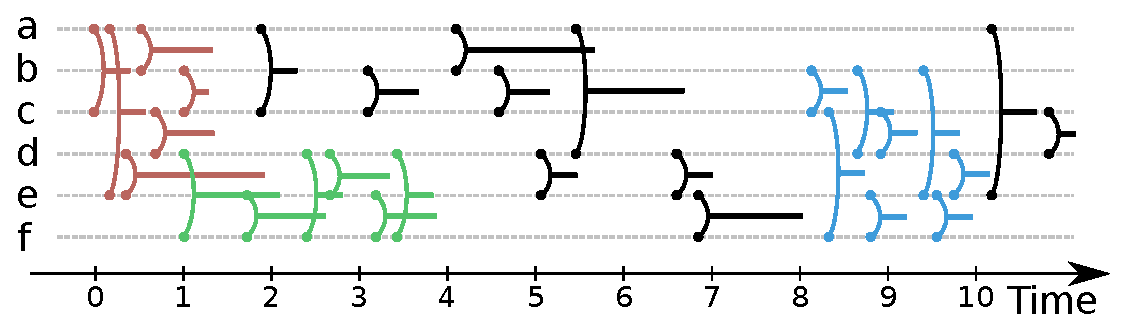
\includegraphics[width=\linewidth]{img/GroupeDense/GroupExample/Zone_dense.eps}
\caption{Exemple de flots de liens avec 3 groupes denses représenté par la couleur des liens (\textcolor{brique}{\textbf{rouge}}, \textcolor{vert_turquoise}{\textbf{vert}} et \textcolor{bleu_window}{\textbf{bleu}}).
}
\label{fig:exemple_groupe_dens}
\end{figure}

\section{Travaux existants}
\label{sec:groupe_dense_existant}

Comme nous l'avons vu dans le chapitre~\ref{chap:etat_art}, il existe assez peu de méthodes cherchant des structures dans un formalisme sans perte d'information.

Mitra~\emph{et al.}~\cite{Mitra2012a} et Speidel~\emph{et al.}~\cite{Speidel2015} ont développé une méthode de détection de communautés mais dans les réseaux diachroniques.
Dans un tel réseau, ce sont les n\oe uds qui ont un \emph{timestamp} et non les liens.
Ce cas de figure s'applique parfaitement aux réseaux de citations car une citation relie bien deux publications apparues à deux dates spécifiques.
Cependant ce genre de situation est particulière et ne peut pas être trivialement représentée par le formalisme de flot de liens.
C'est pourquoi nous ne pouvons utiliser la même méthode. 

Ils existent également des méthodes capturant la partie la plus dense d'un réseau.
C'est le cas de Bogdanov~\emph{et al.}~\cite{Bogdanov2011} qui considèrent  un graphe dont la topologie n'évolue pas mais dont les poids des liens changent entre $-1$ et $1$ en fonction du temps.
Ce formalisme est encore une fois très différent de celui de flot de liens.
De plus, la notion de densité utilisée ne tient pas vraiment compte du temps car un groupe de n\oe uds sur un intervalle est évalué par la somme des liens entre ces n\oe uds sur tout l'intervalle.


Epasto~\emph{et. al}~\cite{Epasto2015} capturent le sous-graphe le plus dense dans un graphe temporel.
Ainsi, le temps est bien pris en compte dans le formalisme.
Cependant, la méthode capture le sous-graphe à un instant $t$ tel qu'il ait le degré moyen le plus élevé parmi l'ensemble des sous-graphes sur tous les instants.
La notion de densité est donc statique car elle ne considère que la structure de graphe à un instant.


Enfin il existe les travaux de Rozenshtein~\emph{et. al}~\cite{rozenshtein2014} qui se rapprochent le plus de notre méthode.
Leur méthode utilise le formalise de flots de liens et ne suppose pas de structure de graphe à un instant donné.
Elle capture un groupe de n\oe uds et plusieurs intervalles disjoints de telle sorte que ce groupe de n\oe uds dans le graphe agrégé sur ces intervalles ait le degré moyen le plus élevé.
plus formellement, un groupe de n\oe uds $V'\subset V$ et un ensemble d'intervalles $\{I_1,..,I_k\} = \mathcal{I} \subset T$ doivent maximiser $\tilde{d}_\mathcal{G}(V')$ où  $\mathcal{G}= \bigcup G(L_t),\,\forall t \in \mathcal{I}$.
Ainsi même si la méthode permet de capturer un groupe de n\oe uds sur des intervalles de temps, elle évalue un candidat sur un graphe agrégé pour appliquer une métrique de graphe.
Le temps n'a donc une influence qu'indirecte sur l'évaluation.
Par ailleurs, leur méthode repose sur plusieurs paramètres qui doivent être fixés \emph{a priori}: le nombre maximum d'intervalles disjoints et la durée cumulée maximum de ces intervalles.
Le premier paramètre permet d'éviter d'utiliser une infinité d'intervalle qui seraient chacun centré sur un lien.
Le second paramètre permet d'éviter de considérer tout le graphe agrégé et ainsi d'imposer la prise en compte du temps.
Ainsi, leur méthode dépend de manière non triviale sur le choix des paramètres.

\bigskip

Pour résumer, il existe des méthodes cherchant la structure la plus dense dans un contexte dynamique; soit en considérant un graphe temporel soit en considérant un flot de liens.
Cependant, ces méthodes utilisent des métriques de graphes pour évaluer un groupe de n\oe uds.
Le temps n'est donc pas complètement pris en compte dans l'évaluation.
De manière plus importante, ces méthodes évaluent de manière absolue un groupe sans prendre en compte son voisinage.
Enfin, nous capturons plusieurs groupes de liens alors qu'ils capturent un groupe n\oe uds.
Certaines de ces méthodes peuvent être étendues pour capturer les $k$ groupes de n\oe uds les plus denses mais cela se fait au prix de l'ajout d'un paramètre pour contrôler le chevauchement entre deux groupes.


\section{Détection de groupes pertinent}
\label{sec:groupe_dense_method}

Nous avons défini dans le chapitre précédent~\ref{sec:fail_mailing} une projection du flot de liens en un graphe statique.
Dans cette projection, chaque lien du flot est représenté par un n\oe ud.
Deux liens $(b,e,u,v)$ et $(b',e',u',v') \in L$ sont reliés dans le graphe s'ils partagent un n\oe ud et si les intervalles s'intersectent, \emph{i.e.} $\{u,v\} \cap \{u',v'\} \neq \emptyset$ et $[b,e]\cap[b',e'] \neq \emptyset$, voir la figure~\ref{fig:Transformation}.
Sur cette projection, nous appliquons l'algorithme de Louvain pour la détection de communautés.
Les communautés trouvées par l'algorithme sont des groupes potentiellement pertinents et nous les appelons donc groupes candidats.

Tous les groupes candidats ne sont pas forcément pertinents.
Tout d'abord, les groupes d'une partition peuvent avoir des tailles très variées.
En particulier, il peut y avoir beaucoup de très petits groupes de $1$ ou $2$ liens.
Ces groupes ne sont pas pris en compte car nous fixons une taille minimum des groupes fixé \emph{a priori}.

Par ailleurs, l'algorithme de Louvain optimise de manière gloutonne la modularité dans la projection du flot de liens en un graphe statique et non une métrique de flot de liens directement.
C'est pourquoi, certains candidats peuvent être une bonne communauté dans le graphe mais un groupe non pertinent dans le flot de liens.
Cet phénomène est d'autant important que la modularité ne prend pas en compte le voisinage d'un groupe.
Par exemple dans la figure~\ref{fig:exemple_groupe_dens}, les liens dans l'intervalle $[4,8]$ forment une composante connexe dans la projection et ils sont considérés comme une communauté par l'algorithme de Louvain.
Or, ces liens ne sont pas un groupe pertinent car ils sont beaucoup moins denses que les liens durant l'intervalle $[0,4]$ ou l'intervalle $[7,11]$.
C'est pourquoi il est nécessaire de filtrer les groupes candidats pour ne garder que les groupes pertinents.




\subsection{Définition des voisinages}
Dans le chapitre~\ref{sec:def_densite}, nous avons défini la densité d'un flot de liens.
Pour un groupe de liens, il faut donc calculer la densité du sous-flot induit par ses liens.
Seulement, la densité en elle même n'est pas un bon critère pour évaluer la pertinence d'un candidat.
En effet, un candidat constitué d'un unique lien a une densité de maximal de $1$.
C'est pourquoi il est également nécessaire de tenir compte du voisinage.
Ainsi, plus le candidat a une densité plus importante que son voisinage, plus le candidat est un groupe pertinent.

Il est donc nécessaire de définir une notion de voisinage qui puisse tenir compte à la fois de la structure et du temps.
Pour ce faire, il faut utiliser une autre formulation de la densité pour comprendre quels sont les paramètres qui influent sur la densité.
Jusqu'à maintenant pour un candidat $C_i$, nous considérons la densité du sous-flot induit par ses liens, $\delta(L(C_i))$.
Pour faire apparaitre l'influence de la structure et du temps, nous utilisons $\delta(L_{\beta(C_i)..\psi(C_i)}(V(C_i)^2))$ que nous simplifions par $\delta(V(C_i),\beta(C_i), \bar{C_i})$ où $\bar{C_i} = \psi(C_i)-\beta(C_i)$.
Il s'agit de la densité des n\oe uds induits par $C_i$ sur la durée du groupe.
Ces deux formulations ne sont pas équivalentes car les deux sous-flots sont différents en particulier $L(C_i) \subseteq L_{\beta(C_i)..\psi(C_i)}(V(C_i)^2)$.
De cette inclusion découle le fait $\delta(L(C_i)) \leq \delta(V(C_i),\beta(C_i), \bar{C_i})$.
C'est le cas dans l'exemple de la figure~\ref{fig:exemple_groupe_dens} si l'on calcule la densité des liens noirs.
Dans ce cas,  tous les n\oe uds sont induits par ces liens et l'intervalle de temps est égale à $[2,11]$.
Le sous-flot induit par $V$ sur $[2,11]$ comprend l'ensemble des liens noirs mais aussi des liens \textcolor{vert_turquoise}{\textbf{verts}} et \textcolor{bleu_window}{\textbf{bleus}}.


Cependant avec cette formulation, on fait apparaitre 3 dimensions: l'ensemble de n\oe uds, le temps de début et la durée.
Il devient alors aisé de considérer comme voisins les sous-flots qui différent sur une seule dimension: soit le temps de début, soit la durée soit l'ensemble de n\oe uds.
Cette différence entre les voisinages est illustrée dans la figure~\ref{fig:voisinage_groupe}.

\begin{figure}
\centering
	\begin{subfigure}{0.31\textwidth}
		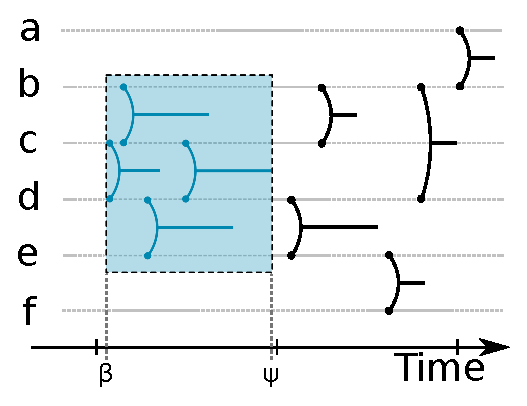
\includegraphics[height=3cm]{img/GroupeDense/GroupExample/Voisinage/Base.eps}
		\caption{Groupe de liens initial}
	\end{subfigure}\hspace*{0.05cm}

	\begin{subfigure}{0.31\textwidth}
		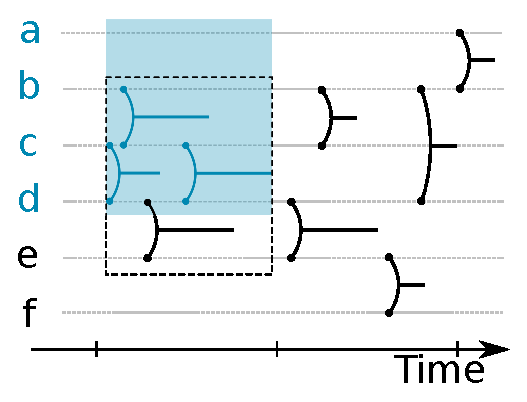
\includegraphics[height=3cm]{img/GroupeDense/GroupExample/Voisinage/Variable_Nodes.eps}
		\caption{Voisinage sur les n\oe uds}
	\end{subfigure}\hspace*{0.02cm}
	\begin{subfigure}{0.31\textwidth}
		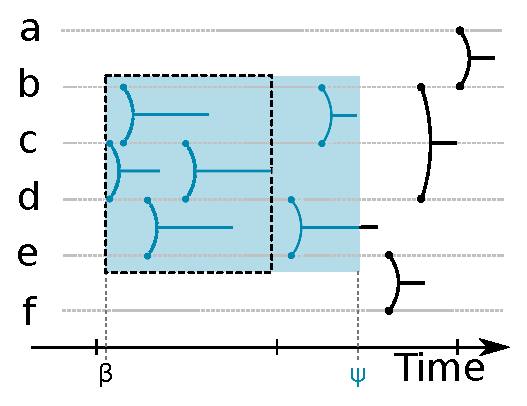
\includegraphics[height=3cm]{img/GroupeDense/GroupExample/Voisinage/Variable_duration.eps}
		\caption{Voisinage sur la durée}
	\end{subfigure}\hspace*{0.02cm}
	\begin{subfigure}{0.31\textwidth}
		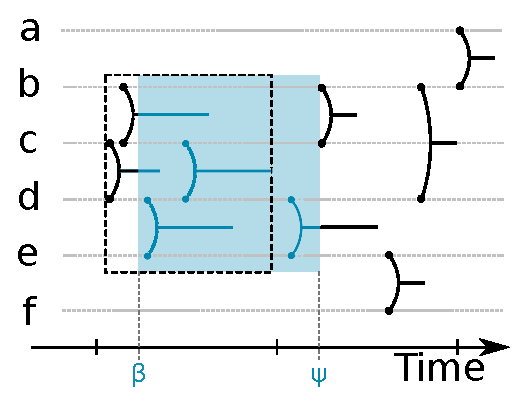
\includegraphics[height=3cm]{img/GroupeDense/GroupExample/Voisinage/Variable_start.eps}
		\caption{Voisinage sur le temps de début}
	\end{subfigure}	
	\caption{Exemple d'un groupe de liens en (A) et de ses différents voisinage en (B), (C) et (D).
	La zone en \textcolor{bleu_transparent}{\textbf{bleu}} est la zone prise en compte lors du calcul de la densité.
	La zone en pointillé représente la zone considérée lors du calcul de la densité du groupe initial.
	}
	\label{fig:voisinage_groupe}
\end{figure}


Pour le voisinage aux n\oe uds, il est impossible de considérer l'ensemble de tous les ensembles de n\oe uds car il est beaucoup trop grand.
De plus, il est probable que ces groupes de n\oe uds ne soient même pas connexe dans le graphe agrégé si le flot de liens est peu dense.
C'est pourquoi, si $V(C_i)$ set constitué de $k$ n\oe uds, nous nous limitons à l'ensemble des groupes de $k$ n\oe uds qui partagent $k-1$ n\oe uds avec $V(C_i)$.
De cette manière, uniquement des groupes de n\oe uds similaires au candidat sont considérés.
Cette comparaison nous semble plus stricte mais plus équitable que celles utilisant l'ensemble des groupes de n\oe uds ou des groupes de n\oe uds pris aléatoirement.
Il serait possible de considérer un nombre moins important de n\oe uds partagés mais nous ne l'avons pas fait à cause de la complexité de calcul.
En effet, il y a déjà $k(|V|-k)$ sous-flots partageant $k-1$ n\oe uds avec un candidat.

Pour le voisinage au temps de début (resp. à la durée), nous considérons toutes les valeurs possibles de temps début (resp. durée) dans un intervalle donné.
Chacune de ces valeurs donne lieu à un sous-flot induit ayant les mêmes n\oe uds et la même durée (resp. temps de début) que le sous-flot induit par les liens du groupe candidat.
Ensuite, nous calculons la densité de chacun de ces sous-flots voisins.
Pus formellement, l'ensemble des densités des sous-flots voisins se défini de la manière suivante.
Soit $I_1$ et $I_2$ deux intervalles et $C_i$ un groupe de liens.
Les densités des sous-flots dans le voisinage au temps de début sont alors définies par la fonction $\delta(V(C_i),x, \bar{C_i})$, $\forall x \in I_1$.
Les densités des sous-flots dans le voisinage de la durée sont alors définies par la fonction $\delta(V(C_i),\beta(C_i), y)$, $\forall y \in I_2$.

L'intervalle utilisé pour le voisinage au temps de début est $[\alpha, \omega-\bar{C_i}]$.
Pour le voisinage à la durée, nous utilisons l'intervalle $[0.8\Delta_{min}, 1.2\Delta_{max}]$, où $\Delta_{min}$ (resp. $\Delta_{max}$) est la plus petite (resp. grande) durée de tous les candidats de plus de 10 liens.
Nous utilisons cet intervalle pour deux raisons.
Tout d'abord, il contient l'ensemble des durées acceptables quand nous l'appliquons à nos jeux de données.
Mais surtout, nous avons également testé l'intervalle $[1-\omega-\alpha]$ qui est beaucoup plus grand.
Cela change les résultat de manière quantitative mais pas de manière qualitative.
En effet lorsque la durée considérée est proche de $\omega-\alpha$ alors la densité est très proche de $0$.
Comme ces valeurs sont peu informatives, nous préférons nous limiter à un intervalle de durée plus restreint.
\bigskip

Au final, nous avons pour chaque voisinage les valeurs de densités des sous-flots voisins.
Pour le voisinage aux n\oe uds, il y a $k(|V|-k)$ valeurs de densité différentes.
Pour le voisinage au temps de début(resp. à la durée), nous avons une fonction de la densité qui dépend du temps de début (resp. de la durée).


\subsection{Définition de l'évaluation}
Nous évaluons chaque candidat en comparant sa densité à celle des sous-flots dans chaque voisinage.
Si un candidat est vraiment pertinent alors il devrait avoir une densité significativement plus élevée que la plupart des sous-flots voisins.
Si les densités des sous-flots voisins suivaient une distribution connue, par exemple une loi normale, alors cela reviendrait à évaluer si la densité du candidat est éloignée de la moyenne en observant le \emph{z-score}.
De par nos observations, les distributions de densités des sous-flots voisins ne suivent pas la même distribution pour différent candidats.
Par exemple dans la figure~\ref{fig:distrib_dens}, des distributions cumulatives de la densité pour le voisinage à la durée pour trois groupes candidats des jeux de donnée Socio Pattern et Rollernet\,\footnote{Ces jeux de données sont présenté dans la section suivante~\ref{sec:groupe_dense_data}.} sont présentées.
Ces distributions sont très différentes et il n'est pas donc pas justifié d'assumer une unique distribution sous-jacente.
C'est pourquoi nous utilisons les \emph{percentiles} qui représentent la proportion des valeurs de densités qui sont inférieures à la densité du candidat.


\begin{figure}
\centering
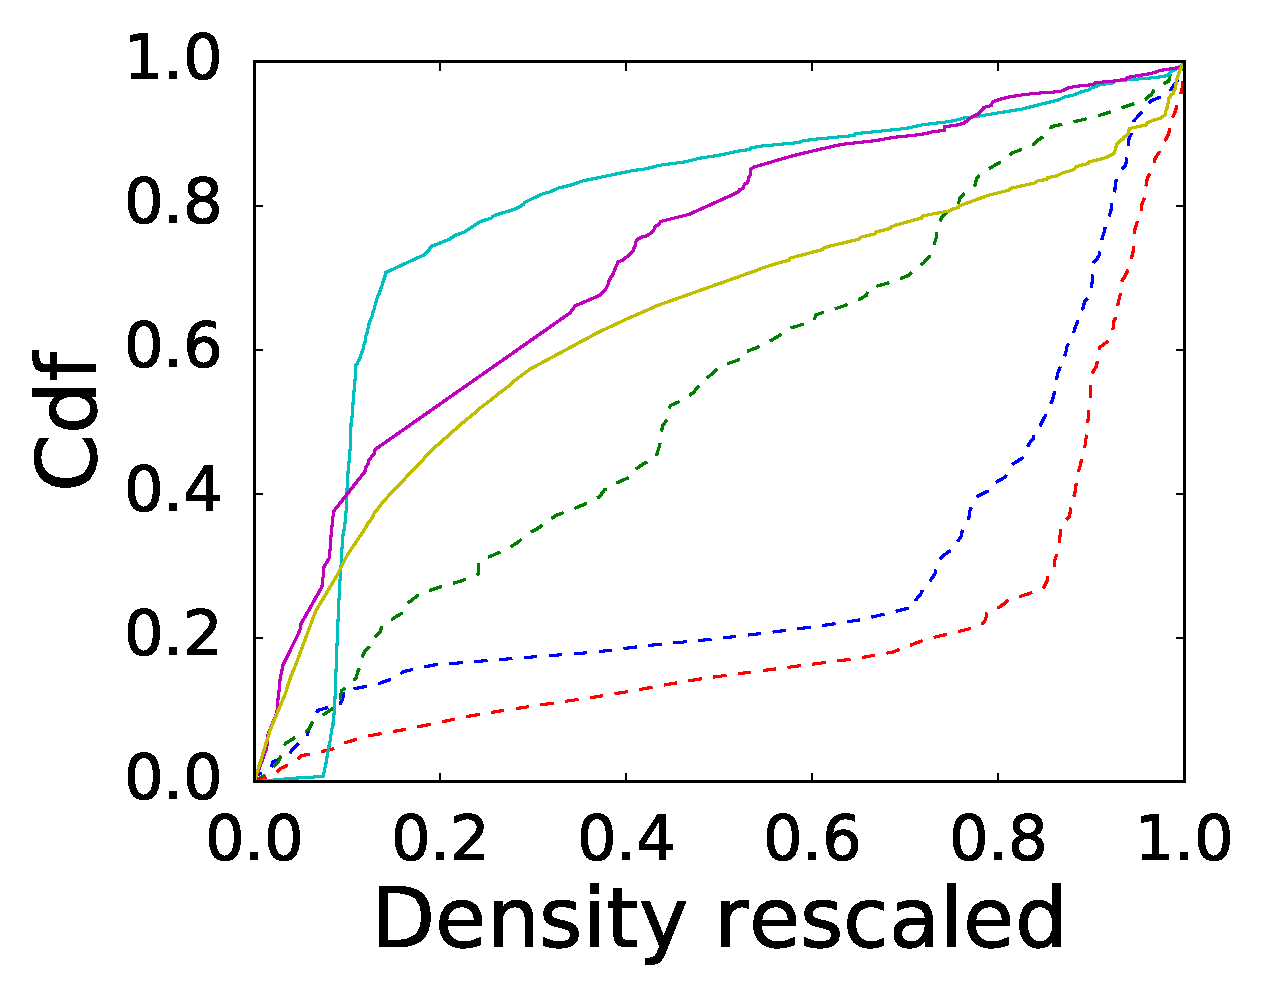
\includegraphics[width=0.3\linewidth]{img/GroupeDense/cdf_density_duration.eps}
\caption{Distributions cumulatives (\emph{cdf}) des valeurs de densité renormalisées des sous-flots voisins dans le voisinages à la durée.
En trait plein (resp. pointillé), trois candidats du jeux de données Rollernet (resp. Socio Pattern).}
\label{fig:distrib_dens}
\end{figure}

Pour le voisinage aux n\oe uds qui est représenté par un ensemble, $S$, de valeurs de densité, le score d'un candidat $C_i$ est:

\begin{equation}
p_{noeud}(C_i)= \dfrac{\sum_{\delta \in S} \mathbf{1}_{\delta \le \delta^*}}{|S|}\,,
\end{equation}
où $\mathbf{1}$ est la fonction indicatrice et $\delta^* =\delta(V(C_i),\beta(C_i), \bar{C_i})$.
Pour les voisinage au temps de début et à la durée qui sont représentés par des fonctions, les scores sont respectivement:

\begin{equation}
p_{d\acute{e}but}(C_i)=\dfrac{1}{\omega-\bar{C_i} - \alpha} \int_{\alpha}^{\omega- \bar{C_i}} \mathbf{1}_{\delta(V(C_i),z,\bar{C_i}) <\delta^*} dz \ ,
\end{equation} 
\begin{equation}
p_{dur\acute{e}e}(C_i)=\dfrac{1}{1.2\Delta_{max} - 0.8\Delta_{min}} \int_{0.8\Delta_{min}}^{1.2\Delta_{max}} \mathbf{1}_{\delta(V(C_i),\beta(C_i),z) <\delta^*} dz \, .
\end{equation}

Un score de $15\%$ pour un voisinage signifie que la densité du candidat est plus faible que $85\%$ des sous-flots dans ce voisinage et que par conséquent le candidat ne devrait pas être considéré comme pertinent.

\bigskip
Pour résumer, un candidat est évalué par un triplet constitué des scores obtenus pour chaque voisinage.
Un candidat est considéré comme pertinent si tous ces scores sont plus élevés que des seuils définis manuellement.
La définition de ces seuils est difficile et dépend des caractéristiques du flot de liens.
C'est pourquoi nous ne les fixons pas \emph{a priori} mais \emph{a posteriori} après avoir examiner la distribution des scores.
Le choix des seuil est décris plus amplement dans la section~\ref{sec:groupe_dense_result}.

\subsection{Algorithme de calcul des scores}
Nous avons défini formellement les trois voisinages mais il faut encore définir un algorithme efficace pour les calculer.
En effet même s'il n'est pas nécessaire de construire explicitement les sous-flots des voisinages, il est nécessaire de considérer l'ensemble des sous-flots.
Cette nécessité est simple à remplir dans le cas du voisinage aux n\oe uds car il existe un nombre fini de sous-flots voisin.
Pour les voisinages au temps de début et à la durée, il existe une infinité de sous-flots voisins car le temps est continu.

\subsubsection{Voisinage aux n\oe uds}
Pour ce voisinage, il est nécessaire d'analyser des sous-flots durant le même intervalle, $[t,t']$, mais pour différents ensembles n\oe uds, $V'$.
Il existe plusieurs stratégies possibles pour calculer la densité  de ces sous-flots. 

La première méthode consiste à manipuler chaque sous-flot de manière indépendante et de calculer leur densité.
Pour extraire le sous-flot induit par un ensemble de n\oe uds sur un intervalle de temps,
il est judicieux de d'abord considérer le sous-flot sur les n\oe uds puis d'intégrer le temps  car la construction du sous-flot induit par un ensemble de n\oe uds est plus rapide.
Le calcul de la densité d'un sous-flot induit par un ensemble de n\oe uds, $V'$ sur intervalle de temps $[t,t']$ est alors dépendant du nombre de liens existant entre les n\oe uds de $V'$ avant $t'$ et de la taille de $V'$: $\tilde{C}_{V'}=O(|L_{\alpha..t'}(V'^2)|log(|V'|))$.
$|L_{\alpha..t'}(V'^2)|$ correspond au parcourt de l'ensemble des liens ayant un de leur n\oe uds dans $V'$ et qui sont potentiellement dans $[t,t']$.
Pour chacun de ces liens, il faut également tester que l'autre n\oe ud du lien appartienne également à $V'$ ce qui se fait en $log(|V'|)$.
Pour calculer l'ensemble du voisinage pour un groupe de n\oe uds de taille $k$, il est alors nécessaire de répéter ce processus pour chaque ensemble de n\oe uds ce qui donne une complexité de $O(k(|V|-k) \tilde{C}_{V'})$.
C'est cette méthode que nous avons implémentée.
Elle est d'ailleurs facilement parallélisable.

La deuxième méthode consisterait en tirer parti de la ressemblance des ensembles de n\oe uds dans le voisinage.
La première étape est alors de calculer $d_{t..t'}(V'^2)$, le degré moyen du groupe de n\oe uds initial.
Puis lors de l'évaluation d'un groupe de n\oe uds voisin $V''$, nous savons que $V'$ et $V''$ ne diffèrent que sur un n\oe ud, $v'$ qui est remplacé par $v''$.
Pour calculer la densité de $V''$ sur $[t,t']$, il suffit de mettre à jour $d_{t..t'}(V'^2)$ en fonction des liens qui ne sont plus pris en compte et des nouveaux liens pris en compte.
C'est à dire qu'il faut considérer $|L_{\alpha..t'}({v'} \cap V')|$ suppressions de liens et  $|L_{\alpha..t'}({v''} \cap V'')|$ ajouts de liens.
Pour évaluer l'ensemble des voisinages, il suffit de répéter ce processus pour chaque groupe de n\oe uds.
Cette méthode peut également être parallélisée.


\subsubsection{Voisinage à la durée}
Pour le voisinage à la duré, l'ensemble de n\oe uds est fixe et il faut de manière continue augmenter la durée du sous-flot voisin.
Pour réussir à faire cela, il est nécessaire de se baser encore une fois sur le degré temporel de l'ensemble de n\oe uds en question.

La densité dépend d'une part de la somme des degrés, $D_{t..t'}(V')$, et d'autre part de la la durée de l'intervalle.
Comme les degrés temporels sont des fonctions constantes par morceaux, la somme des degrés, qui est l'intégrale des degrés, est une fonction linéaire par morceaux dont les points de changement sont les instants où un lien apparaît ou disparaît.
C'est pourquoi, il est possible de définir la densité en fonction de la durée par une fonction par morceaux, voir l'exemple dans la figure~\ref{fig:calcul_var_dure}.
L'idée est de mettre à jour la somme des degrés en fonction de l'apparition et disparition des liens tout en temps compte de la durée du sous-flots qui augmente linéairement.
La complexité est donc $O(|L_{t..t+\Delta_{max}}(V'^2)|)$ si le degré de temporel du groupe est connu.

\begin{figure}
\centering
	\begin{subfigure}{0.4\textwidth}
		\centering
		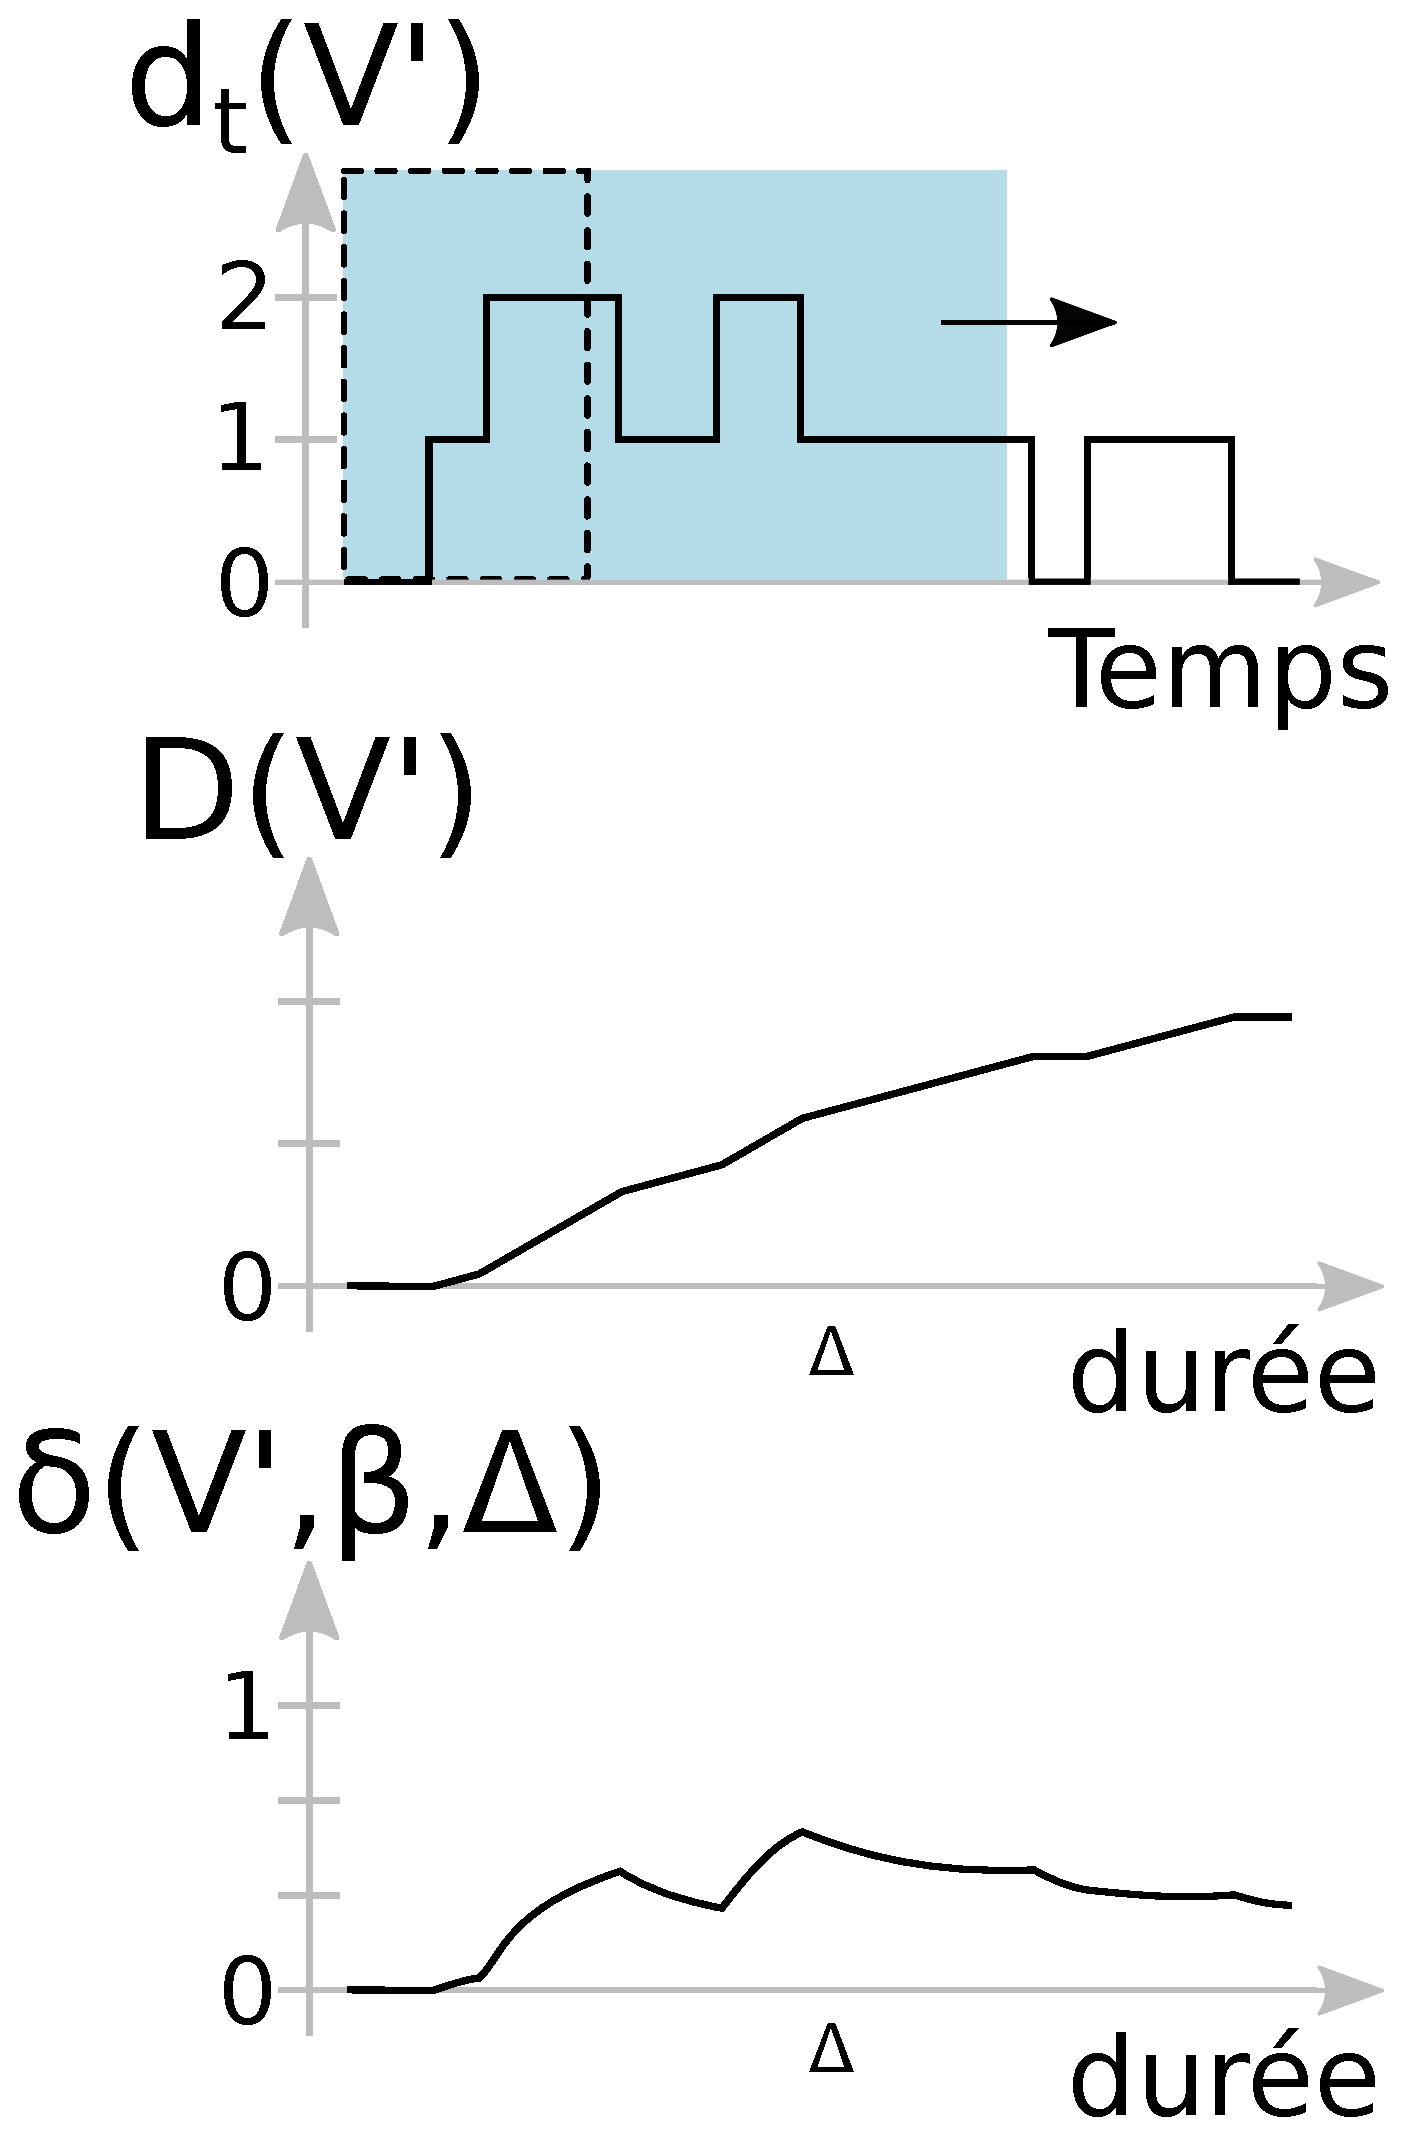
\includegraphics[width=0.8\linewidth]{img/GroupeDense/duration.eps}
		\caption{Voisinage à la durée}
		\label{fig:calcul_var_dure}
	\end{subfigure}\hspace*{0.05\textwidth}
	\begin{subfigure}{0.4\textwidth}
		\centering
		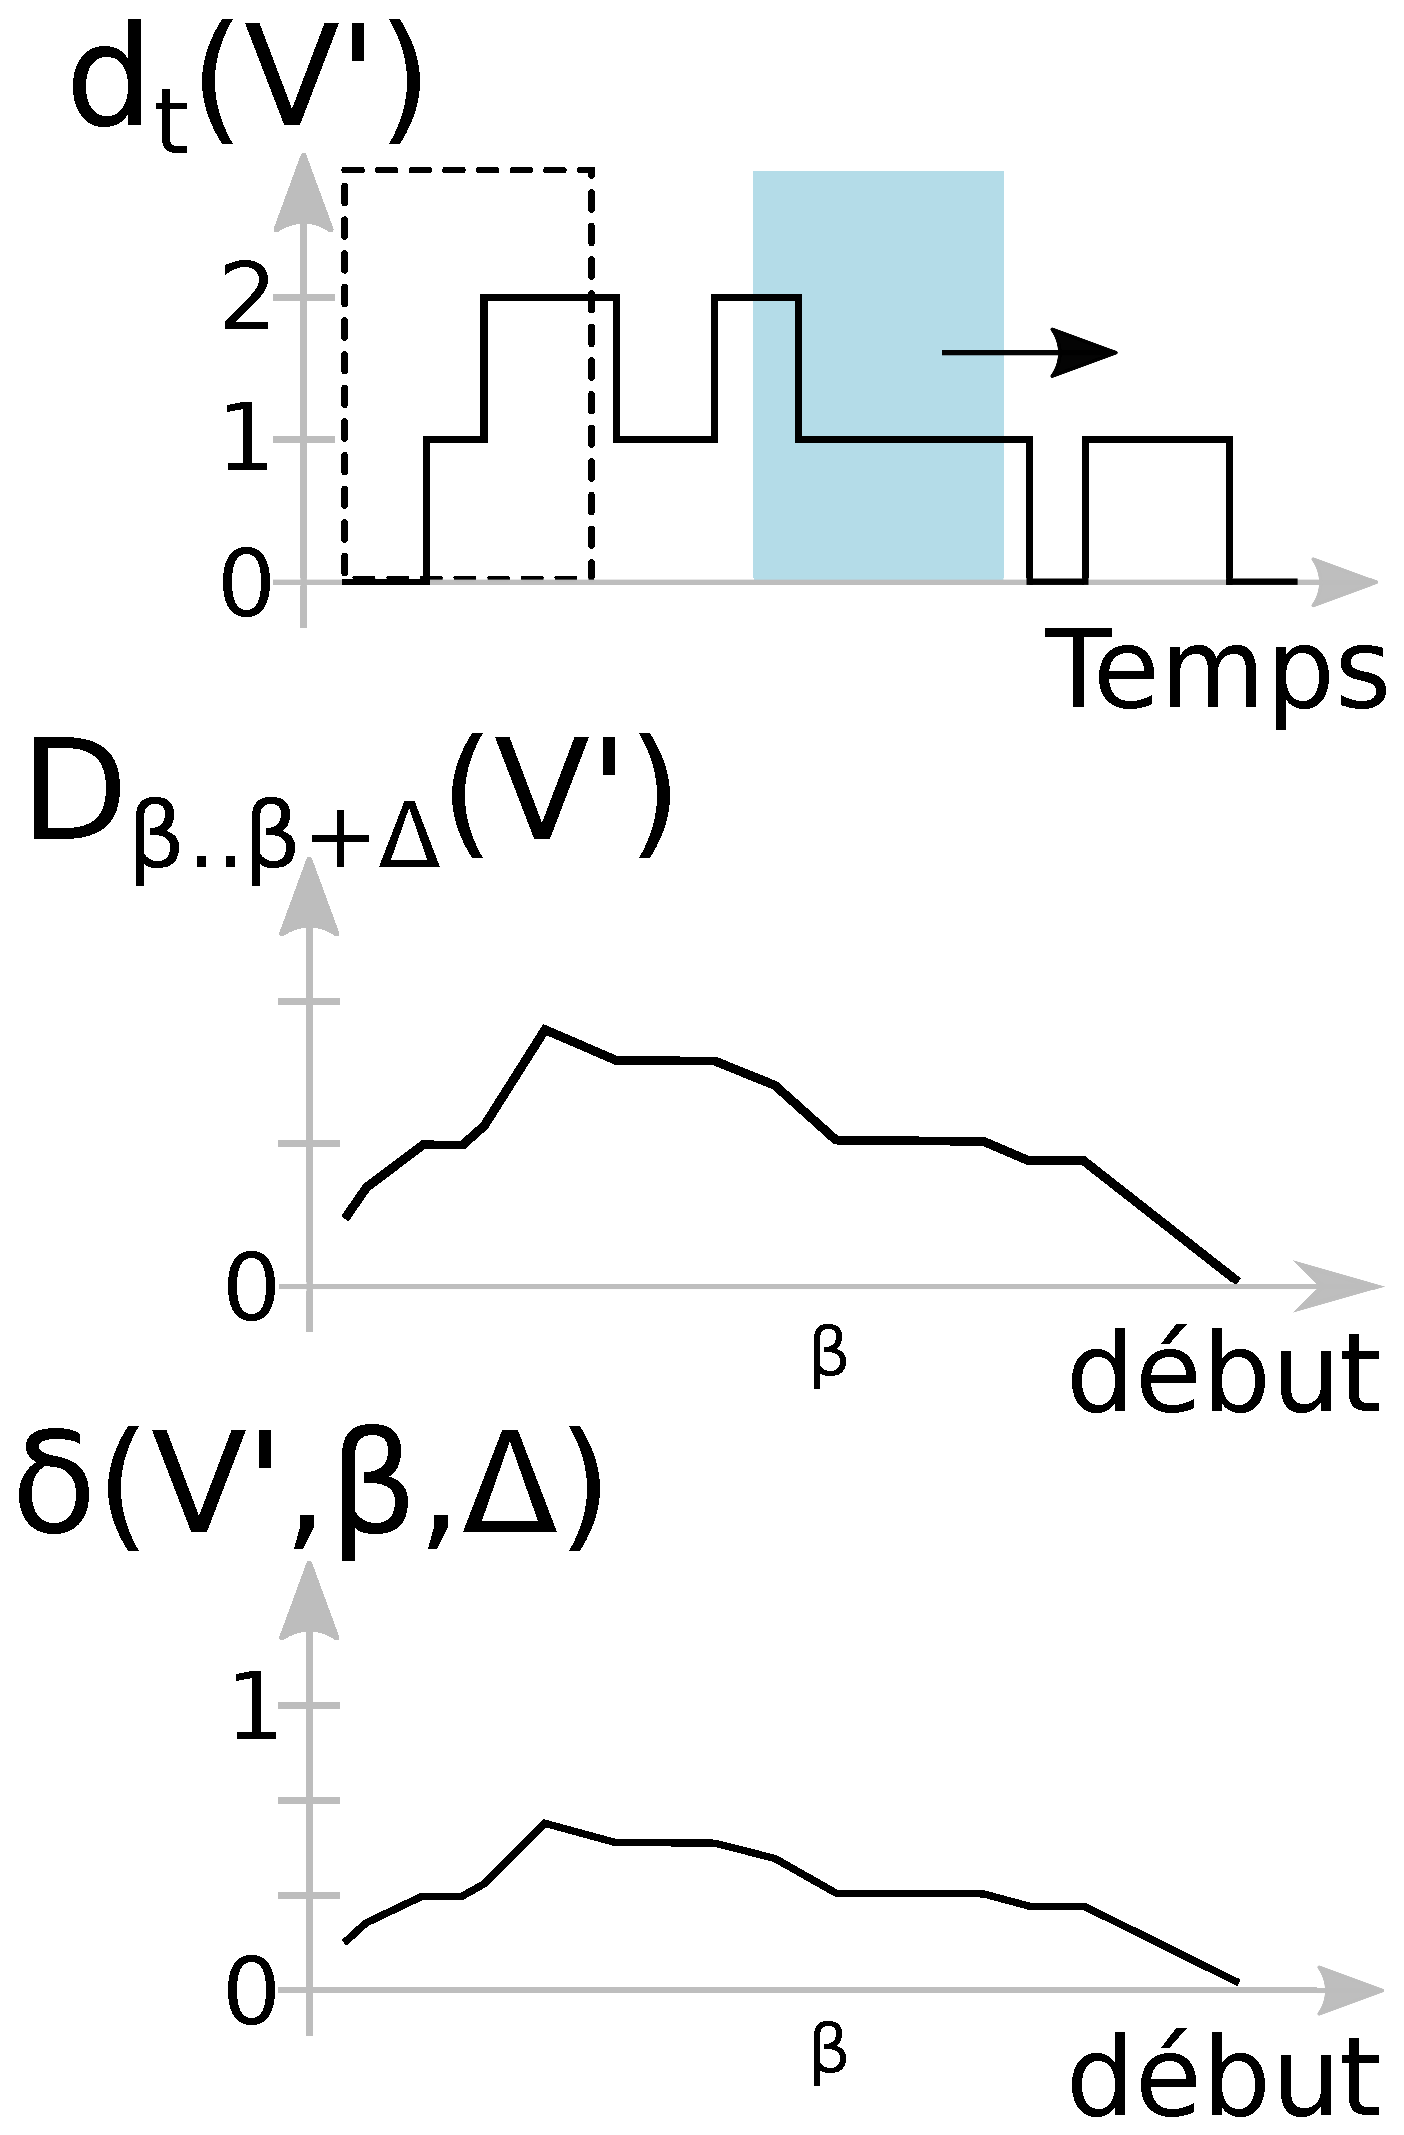
\includegraphics[width=0.8\linewidth]{img/GroupeDense/start_time.eps}
		\caption{Voisinage au temps de début}
		\label{fig:calcul_var_debut.}
	\end{subfigure}\hspace*{0.05cm}

	\caption{Calcul du voisinage à la duré en (A) et au temps de début en (B) pour un groupe ayant un degré temporel donné. Le groupe de liens considéré est le même que celui dans la figure~\ref{fig:exemple_degre}.}
	\label{fig:calcul_var_dure_debut.}
\end{figure}

\subsubsection{Voisinage au temps de début}
Pour le voisinage au temps début, l'approche est similaire.
Il faut mettre à jour la somme des degrés.
La principale différence est que les deux bornes de l'intervalle changent, alors que dans le voisinage à la duré uniquement la borne maximum est modifiée.
Le parcours est donc un peu plus complexe pour calculer $D_{t..t'}(V')$.
Cependant la durée de l'intervalle est fixe, c'est pourquoi il existe une unique bijection entre la somme des degrés et la densité qui est $\delta(V',\beta, \Delta)= \dfrac{D_{t..t'}(V')}{|V'|(|V|-1)}$.
Ainsi, la densité en fonction du temps de début est aussi une fonction linéaire par morceaux.

Voir l'exemple dans la figure~\ref{fig:calcul_var_dure}.
La complexité est donc $O(|L_{\alpha..\omega-\Delta}(V'^2)|)$ où $\Delta$ est la duré du groupe.


\section{Jeux de données}
\label{sec:groupe_dense_data}
Nous appliquons notre méthode sur quatre jeux de données différents.
La table~\ref{tab:data_spec_groupe_dense} liste le nombre de n\oe uds, le nombre de liens et la durée de chaque jeu de données.

\begin{table}
\centering
% table caption is above the table

% For LaTeX tables use
\begin{tabular}{|c|c|c|c|}
\hline  \rule[-1ex]{0pt}{3.5ex}
Datasets & $|V|$ & $|E|$ & $\omega - \alpha$  \\
\hline
Socio Pattern & 180 & 19774 & 9 jours \\
Rollernet & 62 & 15803 &  3 heures\\
Reality Mining & 94 & 44975 & 9 mois\\
Babouins & 28 & 95616 & 14 jours\\
\hline
\end{tabular}
\caption{nombre de n\oe uds $|V|$, nombre de liens $|E|$ et durée de chaque jeu de données.}
\label{tab:data_spec_groupe_dense} 
\end{table}

\begin{description}
\item[Socio Pattern~\cite{Fournet2014}\,\footnote{\url{http://www.sociopatterns.org}}] contient le réseau dynamique d'étudiant d'une classe préparatoire à Marseille en 2012. Durant l'expérience, $180$ étudiants de $5$ classes ont porté pendant $9$ jours des capteurs de proximités.
Ainsi, il est possible de savoir quand deux étudiants interagissent. 
Dans ce jeu de données, la classe de chaque étudiant est connue.\\

\item[Rollernet~\cite{Tournoux2009}] a été collecté durant une randonné roller ayant eu lieu en 2006 à Paris.
Il s'agit d'un événement ayant regroupé $2500$ participants.
Parmi eux, $62$ étaient équipés d'appareils \emph{bluetooth} qui enregistrent l'ensemble des appareils \emph{bluetooth} à portée de communication.
Nous nous limitons uniquement aux contacts ayant eu lieu entre les $62$ personnes portant un capteur.
Des méta-données sont également associées à ces données et notamment le rôle de chaque personne, \emph{e.g.} membre de l'organisation à l'avant du peloton ou membre d'une association de roller.\\

\item[Reality Mining~\cite{Eagle2009}] représente le réseau d'interactions entre $94$ personnes du \emph{MIT Media Laboratory} entre septembre 2004 et juin 2005.
Parmi les $94$ participants, $68$ évoluent dans le même bâtiment (90\% étudiants, 10\% employés) alors que le reste sont des étudiants de l'école de commerce de l'université.
Ce jeu de donné a été récolté grâce à des téléphones \emph{bluetooth} prêtés aux étudiants.\\

\item[Babouins~\cite{Crofoot2015,Strandburg-Peshkin2015}] contient la position \emph{GPS} de $28$ babouins (\emph{Papio anubis}) dans le centre de recherche Mpala au Kenya.
Ces $28$ babouins représentent $80\%$ d'une troupe.
Chaque babouin est équipé d'un collier muni d'un capteur \emph{GPS} qui enregistre la position du babouin toute les secondes.
Nous transformons ces données en un flot de liens en créant un lien entre deux babouins s'ils sont à moins de 1 mètre 50 durant les dernières 10 secondes pour lisser les potentielles imprécisions du \emph{GPS}.
Le code est disponible en ligne\,\footnote{https://bitbucket.org/nGaumont/baboonstreamextractor} et est écris en \emph{rust}.
\end{description}

Même si ces jeux de données sont des réseaux d'interactions face-à-face, ils sont différents dans leur dynamique.
Par exemple, le jeu de données Rollernet a environ le même nombre de liens que celui de Socio Pattern alors qu'il ne dure que trois heures contre 9 jours pour Socio Pattern.
Enfin, nous n'utilisons pas le jeu de données de courriels utilisé précédemment car notre méthode nécessite un flot de liens avec durées.
Nous pourrions utilisé le flot de liens avec des durée ajoutées artificiellement mais elles ne correspondent à aucune réalité.



\section{Application}
\label{sec:groupe_dense_result}

Pour chaque jeu de données, nous appliquons notre méthode pour capturer les groupes d'interactions pertinents.
Comme présenté dans la section~\ref{sec:groupe_dense_method}, la première étape est de trouver une partition, $\mathcal{C}$, des liens.
Quelques statistiques obtenues pour chaque partition sont listées dans la table~\ref{tab:partition_spec_gd}, notamment les nombres de n\oe uds et de liens médians.
La première chose qui est frappante est qu'il existe énormément de très petits groupes.
On remarque également que seul le jeu de données Rollernet se distingue des autres en ayant des groupes plus gros.
Cette différence est probablement due au flot de liens qui contient beaucoup de liens pour une durée de seulement trois heures.

\begin{table}
\centering
\begin{tabular}{|c|c|c|c|}
\hline \rule[-1ex]{0pt}{3.5ex}
Jeux de données & $|\mathcal{C}|$ & $\langle|V|\rangle$  & $\langle|L|\rangle$ \\
\hline
Socio Pattern & 12532 (155) & 2 (9) & 1 (15) \\
Rollernet& 559 (75) & 2 (31) & 1 (194) \\
Reality Mining & 5737 (474) & 2 (12) & 1 (36) \\
Babouin & 37671 (1249)  &  2 (7)  & 1 (16) \\
\hline
\end{tabular}
\caption{$|\mathcal{C}|$: nombre de groupes dans la partition, $\langle|V|\rangle$ médiane du nombre de n\oe uds dans un groupe, $\langle|L|\rangle$ médiane du nombre de liens dans un groupe.
Les valeurs en parenthèses correspondent à la valeur quand uniquement les groupes d'au moins $10$ liens sont pris en compte.}
\label{tab:partition_spec_gd}       % Give a unique label
\end{table}


Afin d'avoir une vision plus précise, nous présentons dans la figure~\ref{fig:distri_group_SP} les distributions cumulatives inverses du nombre de n\oe uds, du nombre de liens, de la durée et de la densité des groupes candidats dans le jeu de données Socio Pattern.
Les distributions sont toutes hétérogènes sauf pour la densité.
Les irrégularités dans la distribution de la densité sont dues aux petits candidats; typiquement un groupe de 2 liens entre 3 n\oe uds a une densité de $0.33$ et un groupe avec un seul lien\,\footnote{Ils représentent $83\%$ de tous les candidats.} a une densité de 1.
Les distributions pour les autres jeux de données sont en appendice pages \pageref{fig:distri_group_rollernet} à \pageref{fig:distri_group_RM} dans les figures~\ref{fig:distri_group_rollernet},\ref{fig:distri_group_baboon} et \ref{fig:distri_group_RM}
Pour ces jeux de données, les distributions du nombre de liens, du nombre de n\oe uds et de la durée sont également hétérogènes mais les distributions de densité sont légèrement moins irrégulières.

\groupcharac{Sociopattern}{Socio Pattern}{SP}{}

Comme les très petits groupes de liens ont un intérêt limité pour décrire un flot de liens, nous commençons par écarter les groupes ayant moins de 10 liens.
Même si cela filtre énormément de groupes, il reste tout de même beaucoup de groupes dont il faut encore évaluer la pertinence.

%\groupcharac{RollernetLim}{Rollernet}{rollernet}
%\groupsPerNode{RollernetLim}{Rollernet}{rollernet}
%\percentile{RollernetLim}{Rollernet}{rollernet}
%\groupcharacFilter{RollernetLim}{Rollernet}{rollernet}



\subsection{\`Evalution des groupes candidats}

Pour séparer les groupes qui sont pertinents des autres, nous utilisons des seuils.
Un candidat est ensuite considéré comme pertinent si ses scores sont au dessus des seuils choisis.
Baisser les valeurs des seuils entraine la capture de plus de groupes comme pertinents mais cela ne change ni les groupes candidats ni leurs scores.
Ainsi, si un groupe est considéré comme pertinent pour un seuil donné alors il le sera également pour tout autre seuil inférieur.
C'est pourquoi les seuils sont fixés après avoir étudié les distributions cumulatives inverses de score pour chaque voisinage.
Ces distributions sont représentées pour le jeux de données Socio Pattern dans la figure~\ref{fig:dit_SP}.
Pour ce jeu de données, les scores sont très élevés, c'est-à-dire proche de $1$, peu importe le voisinage considéré.
On remarque également que les distributions cumulatives inverses chutent toutes à partir d'une valeur de score et nous les utilisons comme seuils.

\percentile{Sociopattern}{Socio Pattern}{SP}{}

Nous utilisons pour le vosinage au temps de début, à la durée et aux n\oe uds les valeurs de seuils suivantes: $0.998$, $0.85$ et $0.98$.
Pour les autres jeux de données, les distributions de scores sont présentées en appendice page \pageref{fig:dit_rollernet} à \pageref{fig:dit_RM} dans les figures~\ref{fig:dit_rollernet},\ref{fig:dit_baboon} et \ref{fig:dit_RM}.
Elles sont similaires à celles obtenues pour Socio Pattern mis à part pour le jeu de données Rollernet dont les scores sont plus faibles.
Cette différence est sûrement due est la structure plus dense du flot de liens globale dans le cas de Rollernet.
Enfin, la table~\ref{tab:thresholds} liste les seuils utilisés pour chaque jeu de données.
\begin{table}
\centering
\begin{tabular}{|c|c|c|c|c|}
\hline \rule[-1ex]{0pt}{3.5ex}
Jeux de données & $p_{noeuds}$ & $p_{d\acute{e}but}$  & $p_{dure\acute{e}e}$  \\
\hline
Socio Pattern & 0.98 & 0.998 & 0.85 \\
Rollernet& 0.9 & 0.7 & 0.6 \\
Reality Mining & 0.97  & 0.98 & 0.8 \\
Babouin & 0.95  &  0.99  & 0.85 \\
\hline
\end{tabular}
\caption{$p_{noeuds}$, $p_{d\acute{e}but}$ et  $p_{dure\acute{e}e}$: seuils utilités pour chaque voisinage.}
\label{tab:thresholds}       % Give a unique label
\end{table}

Un candidat est écarté si un a de ses scores est en dessous du seuil correspondant. 
C'est pourquoi, il est important d'analyser par quels voisinages sont filtrés les groupes.
Les corrélations entre chaque voisinage sont présentées pour le jeu de données Socio Pattern dans la figure~\ref{fig:correlation_SP}.
Les trois voisinages filtrent des candidats différents.
Ils ne sont donc pas redondant.
Même si un score élevé dans un voisinage est souvent corrélé avec un score élevé dans les autres, il arrive qu'un candidat est un score parfait dans un voisinage et un score très faible dans les autres.
Cette situation se matérialise dans la figure~\ref{fig:correlation_SP} par des groupes situés en haut à gauche ou en bas à droite.
Les corrélations entre chaque voisinage pour les autres jeux de données sont présentées en appendice pages \pageref{fig:correlation_rollernet} à \pageref{fig:correlation_RM} dans les figures~\ref{fig:correlation_rollernet},\ref{fig:correlation_baboon} et \ref{fig:correlation_RM}.


\correlation{Sociopattern}{Socio Pattern}{SP}{}

Afin d'illustrer les scores et les groupes pertinents, nous présentons maintenant une analyse manuelle pour deux candidats extraits des jeux de données Socio Pattern et Rollernet.
Nous avons choisi ces jeux de données pour une analyse manuelle car des méta-données sont également associées, ce qui aident la validation des résultats.

\subsubsection{\'Etude manuelle d'un groupe de Socio Pattern}
Dans les données Socio Pattern, la classe de chaque participant est connue et nous connaissons également quand commencent les premiers cours et quand ont lieu les pauses.
Le groupe que nous considérons contient $50$ liens entre $17$ n\oe uds et dure environ 15 minutes, ce qui en fait un des plus gros groupes trouvés.
Comme ce groupe commence à 7h44 le deuxième lundi de la capture, il précède le premier cours de la journée qui a lieu à 8h.
De plus parmi les élèves participants à ce groupe, $16$ font parti de la même classe.
C'est pourquoi il est fort probable que ce groupe corresponde à un regroupement d'élèves avant le premier cours.

Cette analyse est une première étape mais elle ne suffit pas.
En effet, il est possible que ce regroupement ait en réalité concerné d'autres n\oe uds, duré plus longtemps ou même commencé à un autre instant.
C'est pourquoi nous avons développé les notions de voisinages et nous avons calculé les scores associés à ce groupe.

\subsubsection*{Voisinage aux n\oe uds}
Pour ce voisinage, le groupe a un score de $0.987$.
Cela implique que ce groupe a une densité plus importante $98\%$ des sous-flots ayant des n\oe uds similaires et exactement le même intervalle de temps.
Dans le cas de ce groupe à 17 n\oe uds, il y a $2771=17(180-17)$ sous-flots dans le voisinage aux n\oe uds.
Ce score élevé nous permet d'être raisonnablement sûr que cet ensemble de n\oe uds est véritablement important dans cet intervalle de temps

\subsubsection*{Voisinage au temps de début}
Pour ce voisinage, la densité en fonction du temps de début est présentée dans la figure~\ref{fig:g9522_debut}.
Les cycles circadiens sont clairement visibles ainsi que la fin de semaine.
Par ailleurs, on remarque qu'avec une densité de $0.04$ le groupe est plus dense que tous les sous-flots ayant la même durée et les même n\oe uds mais un temps de début différent.
C'est pourquoi le groupe obtient un score de $1$ pour ce voisinage.
Il est donc également pertinent vis-à-vis de ce voisinage.

\subsubsection*{Voisinage à la durée}
Pour finir, le groupe a un score de $0.95$ pour le voisinage à la durée et donc le groupe a capturé une durée  pertinente.
La densité en fonction de la durée des sous-flots voisins est présentée dans la figure~\ref{fig:g9522_duree}.
La densité du sous-flot est légèrement plus importante si une durée plus courte est utilisée.
Ce n'est pas complètement surprenant car la durée du sous-flot impacte la densité.

Par ailleurs, il est important de noter deux chose lorsque l'on observe cette courbe.
Tout d'abord, on se rend compte que considérer des durées plus longue n'est pas vraiment utile.
En effet pour ces jeux de données, la fonction de densité tend vers $0$ lorsque la durée est très longue.
C'est pourquoi, augmenter l'intervalle de durée pris en compte ne fait qu'augmenter les scores sans apporter d'information.
De plus, il est possible, qu'avec avec une durée arbitraire pour définir un sous-flot du voisinage, il n'existe aucun groupe de liens exhibant exactement cette durée.
En effet, un sous-flot induit par un ensemble de n\oe uds, $V'$ sur un intervalle donné, $I$, peut mener à considérer des liens sur seulement une partie de leur durée.
C'est le cas notamment si un lien, $(b,e,u,v) \in E$, relie deux n\oe uds de $V'$ et qu'il commence pendant l'intervalle $I$ mais finisse après.
C'est pourquoi trouver un groupe de liens avec un score parfait pour la durée serait très surprenant.

\bigskip

Enfin, nous avons en sus fait un parcours extensif des densité $d(V(C_i),y,z)$ pour $y \in [\alpha, \omega - \bar{C_i}]$ et $z \in [0.8\Delta_{min}, 1.2\Delta_{max}]$ pour ce groupe en particulier.
Pour ce faire, nous avons dù nous baser sur une discrétisation du temps et n'évaluons $d(V(C_i),y,z)$ que toutes $20$ secondes.
Dans ce contexte, nous obtenons que ce groupe est très souvent le plus dense.

\begin{figure}
\centering
\begin{subfigure}{0.45\linewidth}
	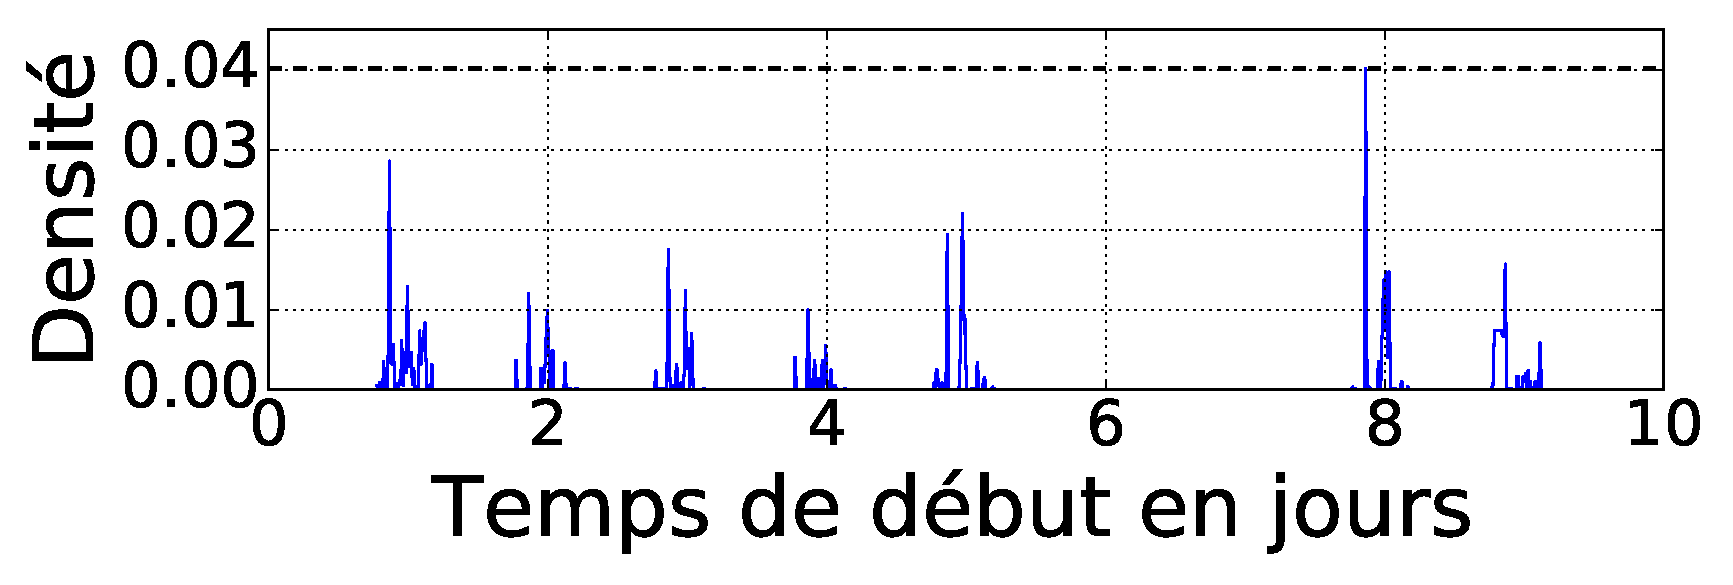
\includegraphics[width=\linewidth]{img/GroupeDense/GroupExample/SocioPattern/vairable_start9522.eps}
	\caption{}
	\label{fig:g9522_debut}
\end{subfigure}
\begin{subfigure}{0.45\linewidth}
	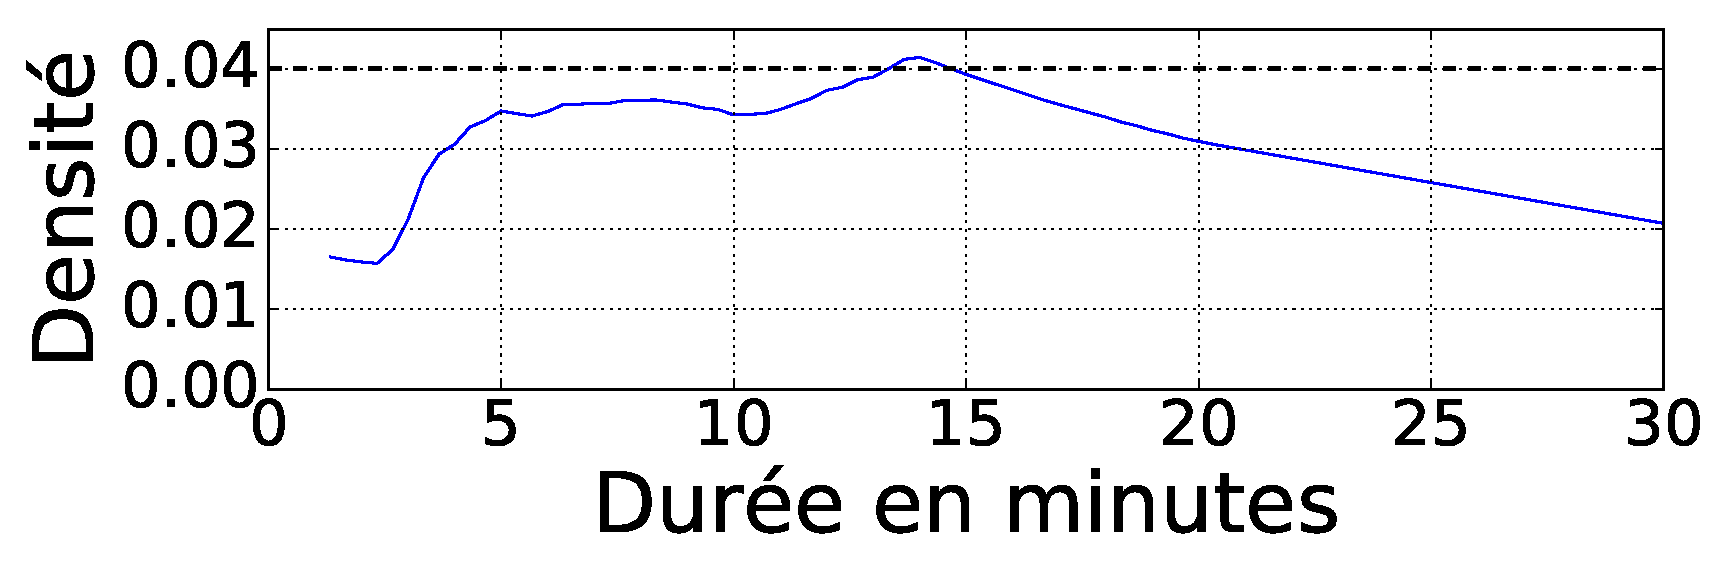
\includegraphics[width=\linewidth]{img/GroupeDense/GroupExample/SocioPattern/vairable_duration9522}
	\caption{}
	\label{fig:g9522_duree}
\end{subfigure}
\caption{
Les figures représentent les densités du voisinage d'un groupe dans Socio Pattern.
En trait plein: la fonction $d(V(C_i),z,\bar{C_i})$ en (A) et la fonction  $d(V(C_i),\beta(C_i),y)$ en (B).
En pointillé, la densité du groupe est rappelée.
}
\label{fig:Sp_g9522_exemple}
\end{figure}

\subsubsection{\'Etude manuelle d'un groupde de Rollernet}
Dans les données Rollernet, nous connaissons le rôle des participants.
Certains des participants ne sont connus que comme membres d'une association de roller mais d'autres ont des rôles plus précis, \emph{e.g.} membre organisateur à l'arrière gauche du peloton.
Ce genre d'information aide lors de l'étude d'un groupe.
Le groupe que nous considérons contient $38$ liens, $9$ n\oe uds et dure pendant environ $5$ minutes.
Ce groupe de liens commence juste au début de la randonnée et $8$ des membres du groupes font parti des membres organisateurs à l'arrière de la randonnée.
Le dernier fait parti des membres organisateurs mais à l'avant.
Ce groupe pourrait indiquer une discussion rapide avant le début du tour.
Comme pour le groupe de Socio Pattern, nous analysons les scores obtenus par ce groupe.


\subsubsection*{Voisinage aux n\oe uds}
Pour ce voisinage, le groupe a un score de $0.99$ ce qui indique une fois de plus que cet ensemble de n\oe uds est important lorsque l'on considère le même intervalle de temps.
Il y a par ailleurs $477=9(62-9)$ sous-flots considérés pour ce candidat dans le voisinage aux n\oe uds.

\subsubsection*{Voisinage au temps de début}
Pour le voisinage au temps de début, le groupe a un score de $0.85$, voir la figure~\ref{fig:g7_debut}.
Comme le jeu de données Rollernet est plus court et plus dense que Socio Pattern, la densité est beaucoup plus stable en fonction du temps de début.
Cela se reflète d'ailleurs sur le score obtenu qui est plus faible.
Cependant comme le groupe de liens en question apparait 5 minutes après le début de la randonnée, il correspond tout de même à un maximum local de la densité.


\subsubsection*{Voisinage à la durée}
Pour le voisinage à la durée, le groupe a un score de $0.86$, voir la figure~\ref{fig:g7_duree}.
Encore une fois, le profil de la densité est plus lisse que dans le cas de Socio Pattern et une durée un peu plus courte donnerait lieu à une densité plus élevée.
Enfin on remarque que, même si Rollernet est beaucoup plus dense que Socio Pattern, la densité décroit tout de même en fonction de la durée considérée.

\bigskip

Même si ces scores ne sont pas optimum et sont plus faibles que ceux obtenus dans l'exemple précédent, il faut les considérer dans le contexte du flot de liens de Rollernet.
Comme Rollernet est globalement plus dense, il est moins surprenant d'observer des sous-flots qui soient denses.
 

\begin{figure}
\centering
\begin{subfigure}{0.45\linewidth}
	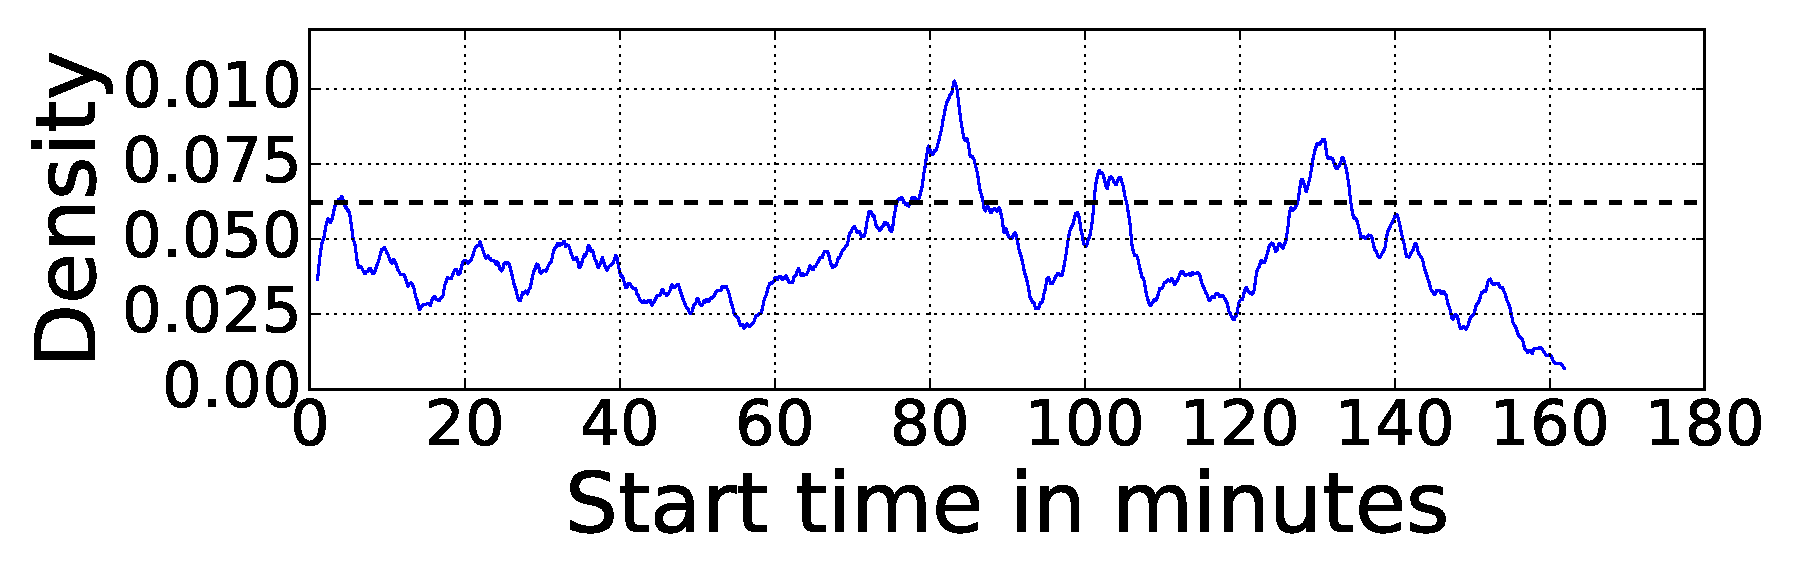
\includegraphics[width=\linewidth]{img/GroupeDense/GroupExample/Rollernet/vairable_start7}
	\caption{}
	\label{fig:g7_debut}
\end{subfigure}
\begin{subfigure}{0.45\linewidth}
	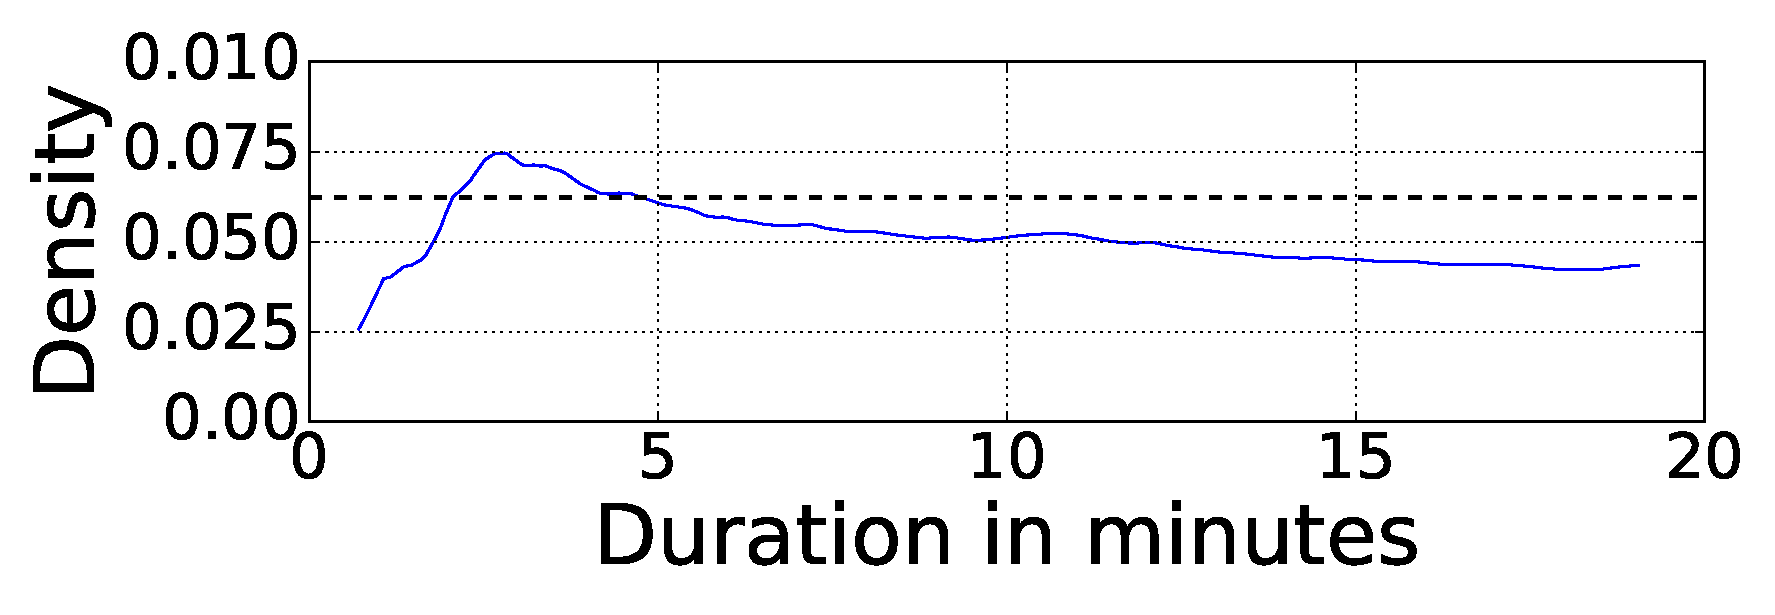
\includegraphics[width=\linewidth]{img/GroupeDense/GroupExample/Rollernet/vairable_duration7}
	\caption{}
	\label{fig:g7_duree}
\end{subfigure}
\caption{
Les figures représentent les densités du voisinage d'un groupe dans Rollernet.
En trait plein: la fonction $d(V(C_i),z,\bar{C_i})$ en (A) et la fonction  $d(V(C_i),\beta(C_i),y)$ en (B).
En pointillé, la densité du groupe est rappelée.
}
\label{fig:Rollernet_exemple}
\end{figure}





\bigskip
Pour résumer, il y a $12 532$  groupes candidats initialement dans le cas de Socio Pattern.
Parmi eux, $155$ ont plus de $10$ liens et $136$ sont considérés comme pertinents.
C'est $136$ groupes représentent $3507$ liens soit $17.7\%$ du flot de liens initial.
Les groupes pertinents sont donc bien une structure partielle du flot de liens.
La table~\ref{tab:res_exec} résume le nombre de final de groupes pertinents capturés pour chaque jeux de données.
On remarque notamment que même si peu de groupes sont capturés, ils représentent une plus grande proportion des liens du flots de liens pour les autres jeux de données.

\begin{table}
\centering
\begin{tabular}{|c|c|c|c|}
\hline \rule[-1ex]{0pt}{3.5ex}
 & $N_c$ & Représentativité  & temps d'exécution \\
\hline
Socio Pattern & 136 & $17.7\%$ & 2 min \\
Rollernet& 37 & $95.4\%$ & 4 min \\
Reality Mining & 394 & $80.9\%$ & 1h \\
Babouin & 1023 & $39\%$ & 52 min\\
\hline
\end{tabular}
\caption{$N_C$ nombre de groupes capturés, proportion de liens appartenant à un groupe pertinent et temps d'exécution pour chaque jeu de données}
\label{tab:res_exec}       % Give a unique label
\end{table}


Tous ces groupes ont des scores plus élevés que les seuils que nous avons fixés mais pour la plupart ils n'ont pas des scores parfaits.
Cela implique qu'il existe des sous-flots voisins ayant une densité plus importante.
C'est pourquoi nous avons également comparé la densité obtenue par le groupe à celle obtenue par le meilleur des sous-flots dans un voisinage donné.
Nous observons que dans $75\%$ des cas la densité des groupes est à moins de $20\%$ de l'optimale.
C'est écart est relativement stable selon les jeux de données et les voisinages.

Les groupes que nous considérons comme pertinent ont donc une densité proche de l'optimum quand bien même cet optimum n'est pas atteignable par un groupe de liens.
De plus, nous avons considéré les voisinages de manière séparée.
Or, il se peut par exemple que le sous-flot optimum dans le voisinage au temps de début ne soit pas l'optimum dans le voisinage à la durée.


\subsection{Caractéristiques des groupes pertinents}

Afin d'avoir une vision plus précises des groupes capturés comme pertinents, nous présentons encore une fois les distributions cumulative inverse du nombre de liens, de n\oe uds, de la durée et de la densité sont présentées dans la figure~\ref{fig:distri_group_SP_filter}.
Les distributions sont encore une fois hétérogènes sauf pour la densité.
Les distributions pour les autres jeux de données sont en appendice pages \pageref{fig:distri_group_rollernet_filter} à \pageref{fig:distri_group_RM_filter} dans les figures~\ref{fig:distri_group_rollernet_filter},\ref{fig:distri_group_baboon_filter} et \ref{fig:distri_group_RM_filter}.
En plus de ces distributions, nous avons également étudié comment ces groupes de liens se répartissent dans le temps et la topologie de l'ensemble du flot de liens.
\groupcharacFilter{Sociopattern}{Socio Pattern}{SP}{}

\subsubsection{Caractéristiques topologiques}
Pour la répartition topologique des groupes, la distribution du nombre de groupes pertinent par n\oe uds est présentée dans la figure~\ref{fig:PropNode_SP} pour le jeu de données Socio Pattern.
Tous les n\oe uds appartiennent à au moins un groupe et quelques n\oe uds appartiennent même à plus de $20$ groupes.
Avec une moyenne de $7.4$ groupes par n\oe uds, les groupes pertinents forment donc une structure très recouvrantes sur les n\oe uds.
Pour les autres jeux données voir les figures~\ref{fig:PropNode_rollernet},\ref{fig:PropNode_baboon} et \ref{fig:PropNode_RM}.
Nous observons également sur ces jeux de données un structure très chevauchante sur les n\oe uds, en particulier pour le jeu de donnée Babouin.
Cette différence est sûrement due au nombre relativement faible de n\oe uds comparé au nombre de liens: $28$ n\oe uds pour $95616$ liens.

\bigskip

Il serait possible que cette structure très chevauchante aurait pu être détectée par une méthode capturant des communautés chevauchantes de n\oe uds dans un graphe.
Enfin de tester cette hypothèse, nous créons un graphe agrégé pondéré tel que le poids d'un lien entre deux n\oe uds soit égale à la somme des durées des liens entre ces deux n\oe uds dans le flot de liens.
Comme l'algorithme de détection de communautés chevauchantes, nous avons utilisé l'algorithme bigclam proposé par Yang~\emph{et al.}~\cite{Yang2013} que nous avons décris dans la section~\ref{subsec:cover}.
Cette méthode ne considère que des graphes non pondérés.
C'set pourquoi il est nécessaire de transformer le graphe pondéré en graphe non pondéré.
Comme aucune valeur singulière de pondération n'est apparue lors de l'étude de la distribution des poids des liens, nous avons avons créé plusieurs graphes non pondérés selon la règle suivante.
Un lien existe dans le graphe non pondéré si le poids associé au lien est plus important ou égale à $\lambda\%$ des poids de tous les liens du graphe pondéré.
Ainsi en faisant varier $\lambda$, il est possible de prendre en compte dans une certaine mesure l'information temporelle.
Une fois les graphes construits, nous appliquons l'algorithme \emph{bigclam} sur chaque graphe et obtenons des partitions chevauchantes de n\oe uds.

Nous utilisons l'indice de Jaccard afin de comparer les partitions chevauchantes obtenues par \emph{bigclam} et celle définie par les n\oe uds induits par les groupes pertinents.
L'indice de Jaccard, défini dans la section~\ref{sec:def_graphe}, nous permet de trouver, pour chaque groupe pertinent, le groupe trouvé par \emph{bigclam} qui est le plus proche.
La table~\ref{tab:Jaccard} liste les similarités médianes et maximums entre les groupes pertinents et ceux trouvés par \emph{bigclam} selon la valeur de $\lambda$ utilisée.
Lorsque l'on étudie cette table, on remarque que les groupes pertinents et les groupes trouvés par \emph{bigclam} sont différents car les indices de Jaccard médians sont très faibles.
Il y a toute fois quelques groupes pertinents qui sont retrouvés par \emph{bigclam} dans certains jeu de données.
Seulement, cela n'arrive que pour quelques valeurs de $\lambda$ et très peu de groupes.
C'est pourquoi notre méthode permet de mettre en valeur une structure des n\oe uds qui n'est pas retrouvée par une méthode classique sur le graphe agrégé.

\begin{table*}
\centering
\begin{tabular}{|c|c|c|c|c|c|c|}
\hline  \rule[-1ex]{0pt}{3.5ex}  & $\lambda= 0.05$ &$\lambda= 0.1$ & $\lambda=0.2$ & $\lambda=0.3$ & $\lambda=0.5$ & $\lambda=0.7$ \\ 
\hline Socio Pattern & 0.30 (0.55)  & 0.30 (0.55)  & 0.30 (0.55)  & 0.30 (0.55)  & 0.29 (0.54) & 0.33 (\textbf{0.85})  \\ 
\hline Rollernet & 0.40 (0.52) & 0.39 (0.64) & 0.41 (0.54) & 0.37 (0.54) & 0.31 (0.57)  &  0.26 (0.75) \\ 
\hline Reality Mining & 0.42 (0.76)  & 0.42 (0.77) & 0.36 (\textbf{0.88}) & 0.42 (\textbf{0.86}) & 0.38 (\textbf{0.87})  & 0.36 (\textbf{1}) \\ 
\hline Baboons & 0.33 (\textbf{0.95}) & 0.38 (\textbf{1}) & 0.40 (\textbf{0.84}) & 0.46 (\textbf{0.94}) & 0.46 (\textbf{0.93}) & 0.44 (\textbf{0.85}) \\ 
\hline 
\end{tabular} 
\caption{Indice de Jaccard médian (et maximum) entre les groupes pertinents et les groupes trouvés par \emph{bigclam} dans le graphe agrégé où les liens ayant un poids inférieur à $\lambda\%$ des liens ont été retirés.
Les indices de Jaccard suppérieurs à $0.8$ sont en gras.}
\label{tab:Jaccard}  
\end{table*}

\subsubsection{Caractéristiques temporelles}
Pour l'aspect temporel, nous avons également étudié le chevauchement temporel entre les groupes pertinents.
Pour ce faire, nous regardons la proportions du temps durant laquelle il n'existe aucun groupe présent.
Pour tous les jeux de données excepté Rollernet, entre $82\%$ et $95\%$ du temps il n'y a aucun groupes présents.
Cette proportion élevée s'explique par la nature des jeux de données qui couvrent de longue périodes, ce qui inclut des nuits où aucun liens n'apparait.
Pour le jeu de donnée Rollernet, cette proportion de temps sans groupe pertinent n'est que de $15\%$.

De manière plus importante, il existe également des instants où plusieurs groupes pertinents sont présents.
Dans le jeu de données Socio Pattern, c'est notamment le cas lors des pauses ou des repas le midi.
Durant ces instants, il peut y avoir jusque quatre groupes présents en même temps.
Ces instants important sont visibles via notre méthode mais ils sont bien évidement facilement identifiable par d'autres méthodes plus simple tel que le degré temporel.

De manière globale, la structure temporelle des groupes pertinents est très différentes de la structure topologique car une part importante du temps n'est impacté par aucun groupe pertinent.
Il est toute fois intéressant de noter que les deux structures sont chevauchantes. 



\section{Conclusion et perspectives}
\subsection{Conclusion}

Dans ce chapitre, nous nous sommes intéressé à la détection de groupes de liens pertinents dans un flot de liens.
\`A l'inverse des méthodes existantes, nous considérons pleinement l'information temporelle et nous n'utilisons aucune agrégation pour évaluer nos résultats.
Cette différence a été permise par l'utilisation du formalisme de flot et de ses métriques mélangeant vraiment structure et temps.
De plus, notre méthode ne capturent pas des ensembles de n\oe uds et des intervalles de temps mais des ensembles de liens.

Pour capturer des groupes de liens, nous avons proposé une transformation du flot de liens en un graphe statique non pondéré tel que les liens sont transformés en n\oe uds dans le graphe.
Deux n\oe uds dans le graphe sont reliés si les liens correspondants dans le flot ont au mois un n\oe ud et un instant de temps en commun.
C'est pourquoi, rechercher une communauté dans le graphe statique permet de trouver des groupes liens connectés temporellement et structurellement.
Nous utilisons l'algorithme de Louvain qui permet de capturer des partitions de n\oe uds dans un graphe.
Nous obtenons ainsi un ensemble de groupes de liens potentiellement pertinents.

Afin de trouver les groupes pertinents parmi l'ensemble des groupes de la partition trouvée par Louvain, nous avons proposé un critère évaluant la pertinence du sous-flot défini par les liens du groupe.
Un sous-flot est jugé pertinent en fonction de scores comparant la densité du sous-flot et la densité des sous-flots proches temporellement et topologiquement.
Un sous-flot peut être caractérisé par les n\oe uds participants à ce sous-flot, l'instant d'apparition du premier lien du sous-flot et la durée du sous-flot.
Il est donc naturel de considérer trois voisinages.
Chaque voisinage est alors composé de sous-flots différant du sous-flot initial sur un seul aspect: l'ensemble de n\oe uds, le temps début ou la durée.
Le score d'un groupe de liens dans un voisinage est ainsi défini par la proportion de sous-flots étant moins denses que lui.
Finalement, le groupe de liens est jugé pertinent si ces scores sont plus élevés que des seuils qui sont fixés \emph{a posteriori}.
Ainsi, modifier ces seuils ne modifient pas les groupes candidats mais uniquement les groupes qui sont jugés pertinents.


Nous avons appliqué notre méthode sur quatre jeux de données réelles représentants des interactions entre individus.
Deux d'entre eux sont des interactions d'étudiant.
Un est un réseau de participant à une randonnée roller à Paris et le dernier est un réseau de babouins.
Ils proviennent ainsi de contextes radicalement différents.
Cela se traduit notamment sur la densité  globale des flots de liens.
Pour tous ces jeux de données, nous avons réussi à capturer des groupes ayant des scores très élevés.

La validation de ces résultats est délicate car il n'existe pas de vérité de terrains sur ces données et il n'existe aucun algorithme similaire.
Cependant il existe des méta-données pour deux des jeux de données.
De cette manière, nous avons pu analyser manuellement quelques groupes considérés comme pertinents par notre méthode.
Nous avons observé que les groupes étudiés correspondaient à des événements existants dans ces jeux de données comme le regroupement d'étudiants avant le premier cours de la semaine.
Nous avons également étudié comment l'ensemble des groupes pertinents se répartissent dans le temps et la topologie du réseau.
Nous avons observé qu'ils sont très chevauchants sur les n\oe uds et sur le temps mais qu'ils concernent cependant qu'une fraction du temps total.


Afin de tester la nouveauté de la structure que nous capturons, nous avons appliqué un algorithme de détection de communautés chevauchantes, \emph{bigclam}, sur le graphe agrégé.
Il apparait que parmi l'ensemble des groupes pertinents seulement quelques un sont retrouvés par \emph{bigclam}.
Ce résultat illustre l'importance de prendre en compte le temps lors de l'étude d'un réseau.


\subsection{Perspectives}

Notre méthode repose sur la projection du flot de liens en un graphe statique, d'une méthode de détection de communauté, une taille de groupe minimum et des seuils qui sont fixé \emph{à posteriori}.
Les axes de recherches associer à ces travaux sont principalement de deux types: l'amélioration de la détection des groupes pertinents et l'amélioration de la validation des groupes détectés.

\subsubsection{Amélioration de la détection des groupes pertinents}
Notre méthode n'est pas encore automatique car il est nécessaire de fixer les seuils des scores et la taille minimum d'un groupe.
La taille minimum ne semble pas être très délicate à choisir.
Il serait intéressant de voir si notre méthode est capable de filtrer automatiquement les petits groupes.
Nous n'avons cependant pas encore poursuivi cet axe de recherche car la prise en compte des petits groupes impacteraient fortement la distribution des scores et donc le choix des seuils.
De plus, les seuils nécessitent déjà une connaissances des données.

C'est pourquoi, il serait intéressant de pouvoir automatiser le choix de seuil.
Lors de l'application de notre méthode, nous avons à chaque fois observée une forte décroissance dans la distribution des scores.
Une méthode prometteuse serait donc de se baser sur la détection de point d'inflexion pour déterminer les seuils.
Il est par exemple possible de détecter les moments où la dérivé seconde est nulle.
Cependant, le comportement que nous avons observé n'est pas forcément universel et il faudrait donc étudier des flots de liens provenant de différents contextes avant de généraliser cette approche.


Il serait également intéressant de remettre en question la méthode de détection utilisée.
Nous utilisons l'algorithme de Louvain sur la projection du flot de liens en un graphe statique
D'une part, il est possible d'utiliser d'autres algorithmes de détection de communautés en tant que partition n\oe uds tels que ceux listés dans la sous-section~\ref{subsec:Part_noeuds}.
Mais il est également possible de considérer les couvertures comme une liste de candidats potentiels.
Il serait par exemple possible d'appliquer \emph{bigclam} sur la projection.
D'autre part, il est également nécessaire de réfléchir l'impact sur les groupes candidats de l'utilisation de la projection du flot en un graphe car il est possible qu'un groupe pertinent ne soit pas détectable dans la projection.
En effet, un lien dans la projection nécessite notamment un chevauchement temporel des liens dans le flot de liens.
Si deux liens sont séparés par un intervalle de temps, alors ils ne seront pas reliés dans la projection peut importe la durée de l'intervalle les séparant.
Il serait donc intéressant de détecter directement les groupes pertinents.

Il n'est pas possible, à partir de la projection, de calculer la densité et les voisinages d'un groupe de lien.
Il est donc nécessaire de manipuler directement un flot de liens pour espérer trouver les groupes pertinents.
Comme l'évaluation d'un groupe de liens est locale, une approche locale intégrant au fur et à mesure des liens dans un groupe candidat est envisageable.
Le but est alors d'améliorer un groupe jusqu'à obtenir un équilibre de Nash, c'est à dire qu'il ne soit pas possible d'améliorer un score sans dégrader les deux autres.
Même si cette approche ne permet pas la détection direct de groupes pertinent, il serait intéressant d'améliorer localement les groupes candidats proposés par l'algorithme de Louvain.


\subsubsection{Amélioration de la validation des résultats}

Nous avons comparé nos résultats à une méthode statique et non la littérature dans les flots de liens car les méthodes de l'état de l'art manipulent principalement des séries de graphes.
La détection de communautés et la recherche de groupes pertinents sont proches mais le changement de formalisme impacte fortement l'objet d'étude.
Dans une série de graphes, il y a une agrégation temporelle.
L'identité d'un lien est donc perdue lors de l'agrégation et il est ainsi délicat de comparer des groupes de liens dans un flot de liens et des groupes de n\oe uds dans une série de graphes.
Pour pouvoir appliquer les méthodes de série de graphes, il est donc d'abord nécessaire de construire une ou plusieurs transformations du flot de lien en série de graphes.
\`A partir de cette série de graphe, il est alors possible d'appliquer les méthodes existantes pour trouver des communautés dans chaque graphe.
Il serait alors intéressant de calculer les scores obtenus par les sous-flots induit par les n\oe uds d'une communauté sur l'intervalle de temps où la communauté à été détectée dans la série de graphes.


Cette approche permettrait de comparer plus en profondeur les résultats mais pas de les valider.
Comme il n'existe pas de données avec une vérité de terrain, une approche prometteuse serait de créer des modèles génératifs de flots de liens permettant de définir des contraintes sur la densité.
Ainsi, il serait alors possible de tester de manière quantitative notre méthode.
Cela permettrait de plus d'ouvrir la voie pour des méthodes de détection de communautés de liens dans les flots de liens.
Nous abordons le problème de la détection de communauté de liens dans les graphes dans le chapitre suivant et nous esquissons des pistes de générations de flots de liens avec une structure dans le chapitre~\ref{versQualite}.